\documentclass[a4paper]{article}
\usepackage[utf8]{inputenc}
\usepackage{graphicx}
\usepackage{tikz}
\usepackage{hyperref}
\usetikzlibrary{shapes,positioning,calc}

\title{Audio Mixer}
\author{Patrick M. Elsen}
\date{\today}

\begin{document}
\maketitle
\tableofcontents

\section{Introduction}

In this project, I attempt to build an audio mixer. This is a device that I need for myself, and have needed for a while. 

\section{Specifications}

\begin{figure}[!h]
\centering  
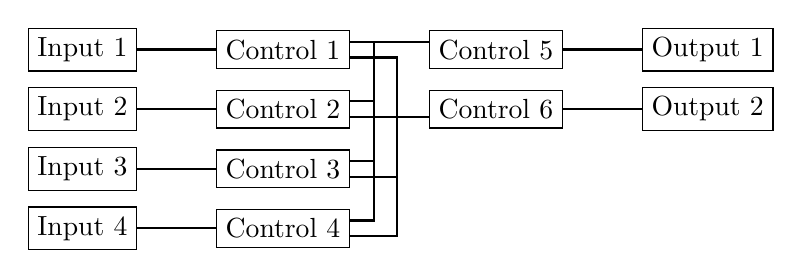
\begin{tikzpicture}
\node[rectangle,draw] (input1) {Input 1};
\node[below=2mm of input1,rectangle,draw] (input2) {Input 2};
\node[below=2mm of input2,rectangle,draw] (input3) {Input 3};
\node[below=2mm of input3,rectangle,draw] (input4) {Input 4};
\node[right=1cm of input1,rectangle,draw] (control1) {Control 1};
\node[right=1cm of input2,rectangle,draw] (control2) {Control 2};
\node[right=1cm of input3,rectangle,draw] (control3) {Control 3};
\node[right=1cm of input4,rectangle,draw] (control4) {Control 4};
\draw[thick] (input1) -- (control1);
\draw[thick] (input2) -- (control2);
\draw[thick] (input3) -- (control3);
\draw[thick] (input4) -- (control4);
\node[right=1cm of control1,rectangle,draw] (control5) {Control 5};
\node[right=1cm of control2,rectangle,draw] (control6) {Control 6};
\draw[thick] ([yshift=1mm]control1.east) -- ++(0.3,0) |-([yshift=1mm]control5.west);
\draw[thick] ([yshift=1mm]control2.east) -- ++(0.3,0) |-([yshift=1mm]control5.west);
\draw[thick] ([yshift=1mm]control3.east) -- ++(0.3,0) |-([yshift=1mm]control5.west);
\draw[thick] ([yshift=1mm]control4.east) -- ++(0.3,0) |-([yshift=1mm]control5.west);
\draw[thick] ([yshift=-1mm]control1.east) -- ++(0.6,0) |-([yshift=-1mm]control6.west);
\draw[thick] ([yshift=-1mm]control2.east) -- ++(0.6,0) |-([yshift=-1mm]control6.west);
\draw[thick] ([yshift=-1mm]control3.east) -- ++(0.6,0) |-([yshift=-1mm]control6.west);
\draw[thick] ([yshift=-1mm]control4.east) -- ++(0.6,0) |-([yshift=-1mm]control6.west);
\node[right=1cm of control5,rectangle,draw] (output1) {Output 1};
\node[right=1cm of control6,rectangle,draw] (output2) {Output 2};

\draw[thick] (control5) -- (output1);
\draw[thick] (control6) -- (output2);
\end{tikzpicture}
\caption{Logic diagram of audio mixer}
\end{figure}


\begin{enumerate}
  \item Takes power from USB or 12V input jack (either one is fine, USB would be nice).
  \item Takes four stereo inputs, ideally as RCA jacks.
  \item Has volume controls for each of the inputs.
  \item Has two separate volume outputs.
  \item Has independent master volume controls for each of the outputs.
  \item Based on the LF353 operational amplifier.
\end{enumerate}

I came up with these specifications because this is what I need: I have multiple devices on my desk, including my desktop Mac Mini, my MacBook Pro, occasionally another laptop and my phone. Each of these devices should be able to send audio to my stereo system, but my stereo is very basic and has only one line-level input.

This device needs to be able to take audio from any of my devices, mix it together, and send it to either my stereo or my headphones.

This device does not need to do any amplification.

I chose the LF353 because it is available in a small but convenient form factor and relatively inexpensive. 

\section{Research}

I did a bit of research while coming up with the specifications. I need to use some software to actually design the schematic and PCB. I also need to source parts, produce the PCB, and assemble the PCB.

\begin{enumerate}
  \item KiCAD (\url{http://www.kicad-pcb.org/}) is my tool of choice for PCB design.
  \item SnapEDA (\url{https://www.snapeda.com/}) has part outlines and models for KiCAD and is free to use.
  \item SeeedStudio (\url{https://www.seeedstudio.com/}) offers PCB manufacture, assembly, and parts that I might use.
\end{enumerate}

It is important that I find good connectors and potentiometers that will last a while.

For the case, I will find ideas after I have designed the PCB, since it is easy to 3D-print a case.

\end{document}